\chapter{Punkt pracy}
Wartości punktu pracy opisane w sekcji \ref{sec:opis} zostały
zweryfikowane. Weryfikacja polegała na prostym sprawdzeniu na jakiej
wartości wyjścia stabilizuje się obiekt przy zadanym sterowaniu.
Eksperyment potwierdził wcześniej opisane wartości, a jego przebieg
obrazuje wykres \ref{fig:pkt_prac}
\begin{figure}
  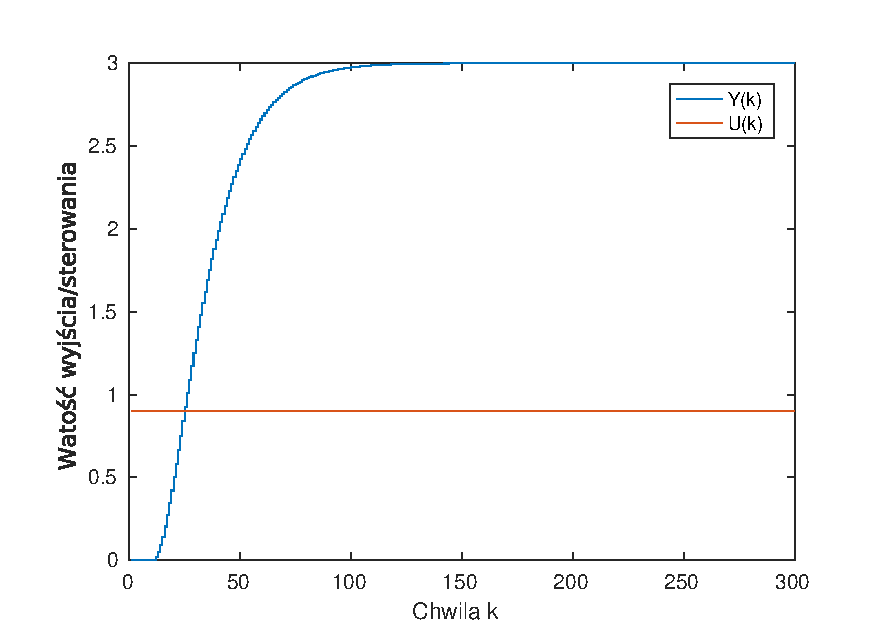
\includegraphics{wykresy/1.eps}
  \caption{Zachowanie obiektu dla stałej wartości sterowania $U = 0.9$}
  \label{fig:pkt_prac}
\end{figure}
